\documentclass[a4paper]{book}

\usepackage[a4paper,top=3cm,bottom=2cm,left=3cm,right=3cm,marginparwidth=1.75cm]{geometry}
%\usepackage{minted}
\usepackage{listings}
\usepackage{scrextend}
\usepackage{enumitem}
\usepackage{float}
\usepackage{amsmath}
\usepackage{hyperref}
\usepackage{todonotes}
\usepackage{etoolbox}
\usepackage[page]{appendix}

\newcommand{\javainline}[1]{\lstinline[language=Java,basicstyle=\ttfamily]{#1}}
\newcommand{\cinline}[1]{\lstinline[language=C,basicstyle=\ttfamily]{#1}}

\makeatletter
\AtEndEnvironment{C}{\xdef\xlang{Language: C}}
\AfterEndEnvironment{C}{\begin{flushright}\vspace{-7mm}\xlang\end{flushright}}
\makeatother

\makeatletter
\AtEndEnvironment{Java}{\xdef\xlang{Language: Java}}
\AfterEndEnvironment{Java}{\begin{flushright}\vspace{-7mm}\xlang\end{flushright}}
\makeatother


\lstnewenvironment{Java}{
    \lstset{
        language=java
      , basicstyle=\ttfamily
      , frame=single
    }}{}
    
\lstnewenvironment{C}{
    \lstset{
           language=C
         , basicstyle=\ttfamily
         , frame=single
        }}{}

\newtheorem{definition}{Definition}

\begin{document}

\title{A Bounded Verification Tool for Java}
\author{Stefan Koppier}
\maketitle

\chapter*{Introduction}

\tableofcontents

\chapter{Features}
The tool supports

\section{Unsupported language features}
We provide a comprehensive list describing each language feature that is not 
supporte by the tool. Note that if the reader is reading this document in a pdf 
viewer, the names of the lists provide a link to sources for more information
about the missing part.

\subsection{Object-oriented paradigm}
No support for object-oriented concepts, except for the declaration of classes.
The following three concepts are the main ones that are not supported. Anything
that is built upon these conceps, e.g. calling a base class constructor, is also
not supported.

\begin{labeling}{abstract classes}
\item [\href{https://docs.oracle.com/javase/tutorial/java/concepts/inheritance.html}
            {inheritance}] Inheritance of a class or interface.
\item [\href{https://docs.oracle.com/javase/tutorial/java/concepts/interface.html}
            {interfaces}] An interface declaration.
\item [\href{https://docs.oracle.com/javase/tutorial/java/IandI/abstract.html}
            {abstract classes}] A class or method without an implementation.
\end{labeling} 

\subsection{Statements}
\begin{labeling}{synchronized statements}
\item [\href{https://docs.oracle.com/javase/tutorial/java/nutsandbolts/while.html}
            {do while loops}] \javainline{do \{ \} while(guard)}
\item [\href{https://docs.oracle.com/javase/tutorial/java/nutsandbolts/for.html}
            {for iterator loops}] \javainline{for (int item : numbers) \{ \}}
\item [\href{https://docs.oracle.com/javase/tutorial/essential/concurrency/locksync.html}
            {synchronized statements}] \javainline{synchronized(x) \{ \}}
\end{labeling}

\subsection{Expressions} 
\begin{labeling}{lambda expressions}
\item [\href{https://docs.oracle.com/javase/tutorial/java/javaOO/lambdaexpressions.html}
           {lambda expressions}] \javainline{(x) -> x*x}
\item [\href{https://docs.oracle.com/javase/tutorial/java/IandI/subclasses.html}
           {casting}] \javainline{(int)3.0}
\item [\href{https://docs.oracle.com/javase/tutorial/java/nutsandbolts/op2.html}
           {instance of}] \javainline{x instanceof Integer}
\item [\href{https://docs.oracle.com/javase/tutorial/java/javaOO/methodreferences.html}
           {method reference}] \javainline{Foo::bar}
\end{labeling}

\subsection{Others}
\begin{labeling}{static initialization blocks}
\item [\href{https://docs.oracle.com/javase/tutorial/java/javaOO/initial.html}
            {static initializer blocks}] Static block execution, which should be executed 
when the class is loaded.
\item [\href{https://docs.oracle.com/javase/tutorial/java/javaOO/initial.html}
            {static field initializer}] Static class field initialization, which should
be assigned when the class is loaded.
\item [\href{https://docs.oracle.com/javase/tutorial/java/javaOO/nested.html}
            {nested class definitions}] Class declarations inside classes or inside methods.
\item [\href{https://docs.oracle.com/javase/tutorial/java/generics/index.html}
            {generics}] Generic types, of any kind.
\item [\href{https://docs.oracle.com/javase/tutorial/java/javaOO/enum.html}
            {enums}] Enum declarations.
\end{labeling}

\chapter{On the semantical differences between Java and C}

\section{Types}
The supported Java subset consists of three kind of types: primitives, 
(multi-dimensional) arrays, and classes.

In Java, primitives are stack-allocated, and arrays and classes are heap-allocated.
This requires primitives to be treated as plain types, and arrays and objects to
be treated as pointers.

\subsection{Primitive data types}
Java defines eight primitive data types: \javainline{boolean}, 
\javainline{char}, \javainline{byte}, \javainline{short}, \javainline{int},
\javainline{long}, \javainline{float}, and \javainline{double}. All integral 
values are signed.

C defines one boolean type: \cinline{\_Bool}, five standard signed integer types: 
\cinline{signed char}, \cinline{short int}, \cinline{int}, \cinline{long int},
\cinline{long long int}, and three standard floating point types: \cinline{float},
\cinline{double}, and \cinline{long double} \cite[p.~40]{iso_c_standard}. The 
downside of the integral primitives is that their size is not exactly specified, 
and is thus implementation specific. For example, the \cinline{int} primtive can
be 32- or 64-bit, depending on the implementation. Luckily, CBMC defines four
exact sized integral values: \cinline{\_\_int8}, \cinline{\_\_int16}, 
\cinline{\_\_int32}, and \cinline{\_\_int64} \cite[p.~39]{cprover_manual}.

We can define an exact mapping of the primitve data types of Java, to those of
C and CBMC. This mapping can be found in \ref{table:primitve_data_type_conversions}.

\begin{table}[H]
    \centering
    \caption{Mapping of the primitive data types.}
    \label{table:primitve_data_type_conversions}
    \begin{tabular}{lll}
    \hline
    \textbf{Type}        & \textbf{Description}                 & \textbf{C equivalent} \\ \hline
    \javainline{boolean} & true or false                        & \cinline{\_Bool}      \\
    \javainline{char}    & 16-bit Unicode value                 &                       \\
    \javainline{byte}    & 8-bit signed integral value          & \cinline{\_\_int8}    \\
    \javainline{short}   & 16-bit signed integral value         & \cinline{\_\_int16}   \\
    \javainline{int}     & 32-bit signed integral value         & \cinline{\_\_int32}   \\
    \javainline{long}    & 64-bit signed integral value         & \cinline{\_\_int64}   \\
    \javainline{float}   & IEEE 754 32-bit floating point value & \cinline{float}       \\
    \javainline{double}  & IEEE 754 64-bit floating point value & \cinline{double}      \\ \hline
    \end{tabular}
\end{table}

\subsection{Arrays}
Both Java and C have a concept of an array, but they are vastly different. In 
Java an array is an heap-allocated structure, in C an array is a stack-allocated 
structure, unless it explicitly allocated on the heap. The length of an array is
contained in the Java array structure, this needs to be maintained explicitly in 
C.

To ease both differences, the choice is made to map the Java type of an array 
to a C struct, containing the elements in the array and the length of the array.

For example, the type \javainline{int[]} will be mapped to:
\begin{C}
struct Int_Array {
    __int32 *elements;
    __int32 length;
};
\end{C}

Multi-dimensional arrays are mapped in the same way. For example, the type 
\javainline{int[][]} will be mapped to:

\begin{C}
struct Int_Array {
    __int32 *elements;
    __int32 length;
};

struct Int_Array_Array {
    struct Int_Array **elements;
    __int32 length;
};
\end{C}

\subsection{Classes}
There is no direct translation of a Java class to a C class, as C does not have 
the concept of a class. A Java class consists of three components:

\begin{labeling}{Constructors}
    \item [Fields] Fields can be divided in two sets, non-static fields, which 
    are part of an instantiation of the class, and static fields, which are not
    part of an instantiation.
    \item [Methods] Methods can also be divided in two sets, non-static methods,
    which have an hidden \javainline{this} parameter to the object the method is
    called on, and static methods, which are not called on a specific object. 
    \item [Constructors] The constructors are always static, and return an object
    of the type the constructor is defined in.
\end{labeling}

The class will be mapped to a struct declaration, containing all non-static
fields of that class. All static fields will be mapped to a global variable 
declaration. In the mapping to C, methods and constructors are no longer part of 
the type itself, but a method will be declared for each invocation. The mapping 
of methods and constructors is be described in \todo{reference the mapping of methods.}.

For example, given the following class \javainline{Foo}, without its method and 
constructor declarations:

\begin{Java}
class Foo {
    static bool b;
    int x;
}
\end{Java}

will be mapped to the following declarations in C

\begin{C}
_Bool Foo_b;

struct Foo {
    __int32 x;
};
\end{C}

\section{Expressions}

\subsection{Literals}

\subsection{Operators}

\subsection{Assignment}

\subsection{Method invocation}

\subsection{Array creation}


\section{Statements}

\chapter{The phases of the tool} \label{chap:phases}
The tool consists of five main phases: parsing, control flow analysis, 
linearization, compilation and verification. A global overview of all these phases
and their inputs and outputs can be found in figure \ref{fig:phases_overview}.

\begin{figure}[H]
    \caption{An overview of the phases of the tool.}
    \centering
    \label{fig:phases_overview}
    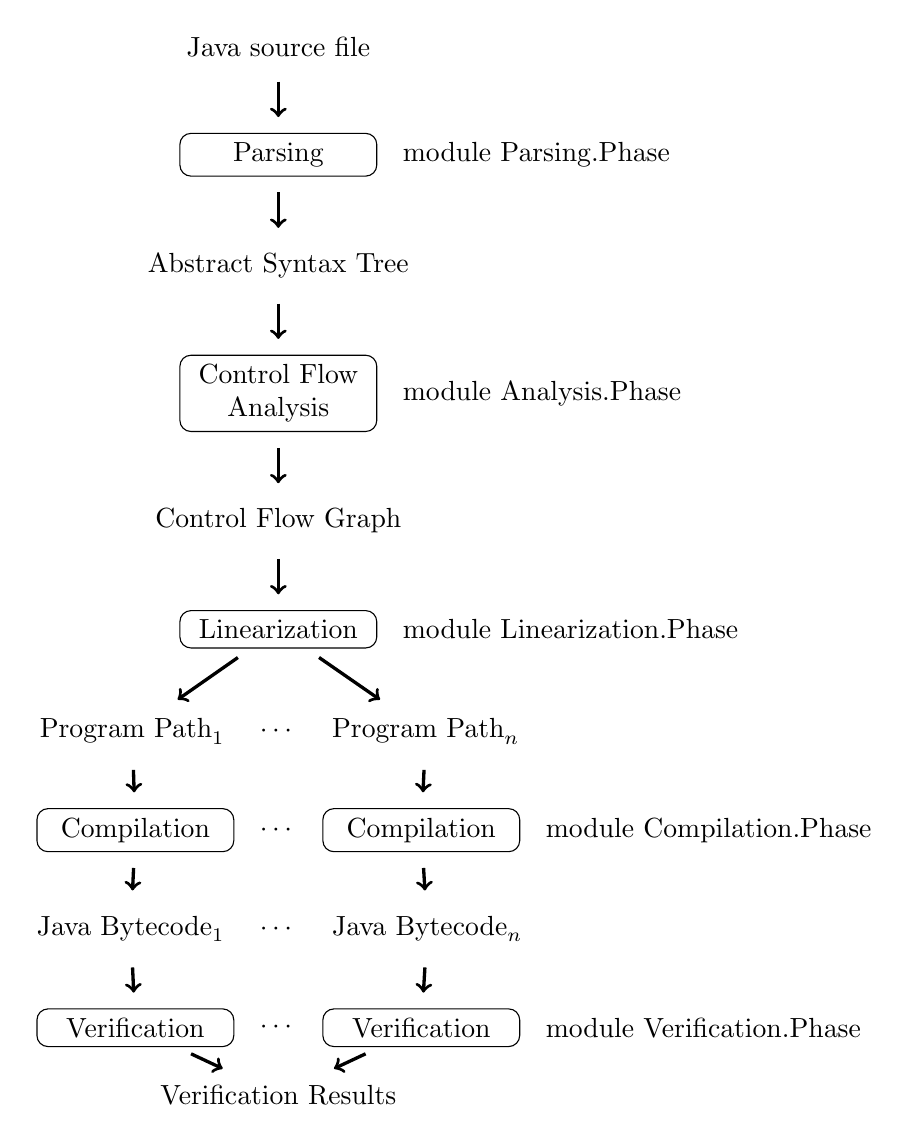
\begin{tikzpicture}[node distance=0.85cm and 0.2cm, align=center]
        \tikzset{
            phase/.style      = { rectangle
                                , rounded corners 
                                , minimum width=2.5cm
                                , text centered
                                , draw=black
                                }
        , intermediate/.style = { rectangle
                                , minimum width=2.5cm
                                }
        , dots/.style         = { rectangle
                                , minimum width=0.5cm
                                }
        , arrow/.style        = { very thick
                                , shorten >= 0.2cm
                                , shorten <= 0.2cm
                                }
        }

        \node(input)             [intermediate]                       {Java source file};
        \node(parser)            [phase,below=of input] {Parsing};
            \node() [right=of parser] {module \haskellinline{Parsing.Phase}};
        \node(ast)               [intermediate,below=of parser]   {Abstract Syntax Tree};
        \node(analyzer)          [phase,below=of ast]    {Control Flow\\Analysis};
            \node() [right=of analyzer] {module \haskellinline{Analysis.Phase}};
        \node(cfg)               [intermediate,below=of analyzer]    {Control Flow Graph};
        \node(linearizer)        [phase,below=of cfg]              {Linearization};
            \node() [right=of linearizer] {module \haskellinline{Linearization.Phase}};
        \node(path_dots)         [dots,below=of linearizer]      {$\cdots$};
        \node(path_1)            [intermediate,left=of path_dots] {$\text{Program Path}_1$};
        \node(path_n)            [intermediate,right=of path_dots] {$\text{Program Path}_n$};
        \node(compiler_dots)     [dots,below=of path_dots]      {$\cdots$};
        \node(compiler_1)        [phase,left=of compiler_dots] {Compilation};
        \node(compiler_n)        [phase,right=of compiler_dots] {Compilation};
            \node() [right=of compiler_n] {module \haskellinline{Compilation.Phase}};
        \node(bytecode_dots)     [dots,below=of compiler_dots]      {$\cdots$};
        \node(bytecode_1)        [intermediate,left=of bytecode_dots] {$\text{Java Bytecode}_1$};
        \node(bytecode_n)        [intermediate,right=of bytecode_dots] {$\text{Java Bytecode}_n$};
        \node(verification_dots) [dots,below=of bytecode_dots]      {$\cdots$};
        \node(verification_1)    [phase,left=of verification_dots] {Verification};
        \node(verification_n)    [phase,right=of verification_dots] {Verification};
            \node() [right=of verification_n] {module \haskellinline{Verification.Phase}};
        \node(results)           [intermediate,below of=verification_dots] {Verification Results};

        \draw[arrow,->] (input) -- (parser);
        \draw[arrow,->] (parser) -- (ast);
        \draw[arrow,->] (ast) -- (analyzer);
        \draw[arrow,->] (analyzer) -- (cfg);
        \draw[arrow,->] (cfg) -- (linearizer);
        \draw[arrow,->] (linearizer) -- (path_1);
        \draw[arrow,->] (linearizer) -- (path_n);
        \draw[arrow,->] (path_1) -- (compiler_1);
        \draw[arrow,->] (path_n) -- (compiler_n);
        \draw[arrow,->] (compiler_1) -- (bytecode_1);
        \draw[arrow,->] (compiler_n) -- (bytecode_n);
        \draw[arrow,->] (bytecode_1) -- (verification_1);
        \draw[arrow,->] (bytecode_n) -- (verification_n);
        \draw[arrow,->] (verification_1) -- (results);
        \draw[arrow,->] (verification_n) -- (results);
    \end{tikzpicture}
\end{figure}

All phases are chained into one phase, the Complete phase. This phase is defined
in the \haskellinline{Complete} module and is the main API of the tool.

\section{Lexing and Parsing}
Lexing and parsing is the first phase of the tool. It consists of two subphases:
the lexer and parser, and the syntax transformation. The complete phase takes a 
\haskellinline{String} as input, and transforms it to a \haskellinline{CompilationUnit'}
defined in the \haskellinline{Parsing.Syntax} module. The 
\haskellinline{CompilationUnit'} can be seen as the root node of the abstract
syntax tree.

The lexing and parsing is done using an intermediate abstract syntax tree, defined
in the library \href{http://hackage.haskell.org/package/language-java}{language-java}.
This library also contains the lexer and parser that is used within the tool.

The output of the parser of the 
\href{http://hackage.haskell.org/package/language-java}{language-java} library 
is fed into a syntax transformation subphase. This phase transforms the abstract 
syntax tree of the \href{http://hackage.haskell.org/package/language-java}{language-java} 
library into the abstract syntax tree defined in \haskellinline{Parsing.Syntax}.
Our abstract syntax tree is almost an one-to-one correspondence of the abstract
syntax tree defined in \href{http://hackage.haskell.org/package/language-java}{language-java}.

The definitions in \haskellinline{Parsing.Syntax} are contained in an attribute 
grammar file, which can be built using the Attribute Grammar System of Utrecht
University\footnote{\url{hackage.haskell.org/package/uuagc}}. This system allows
easy information retrieval of the abstract syntax tree, but at the cost that we
cannot use the abstract syntax tree defined in the 
\href{http://hackage.haskell.org/package/language-java}{language-java} library 
directly.

\subsection{The supported subset of Java}
Only a subset of the Java language is supported. There is support for a single
Java source file containing one or more class declarations. Interfaces and enum 
declarations are not supported. 

Classes may contain fields, methods and constructors. All modifiers on these 
levels are supported, including annotations. Classes may not contain generics, 
note that JBMC also does not have support for generics. Methods and constructors
may not be overloaded, there cannot exist two methods with the same name in the
same class.

Methods and constructors contain statements, of which we distinct two types. 
Compound statements, and basic statements. Compound statements are statements 
which itself contain statements. Basic statements are statements which do 
not contain statements. A constructor may not call its base constructor explicitly.
The compound statements that are supported are:

\begin{itemize}
    \item A block, introduced using curly braces;
    \item an \javainline{if else} statement;
    \item a \javainline{while} loop;
    \item a \javainline{try catch finally} statement;
    \item a \javainline{for} loop.
\end{itemize}

Note that \javainline{while}- and \javainline{for} loops can be labeled, e.g.
\javainline{l: while(g)}.

The basic statements that are are supported are:

\begin{multicols}{2}
    \begin{itemize}
        \item A variable declaration;
        \item a skip statement;
        \item an expression statement;
        \item an \javainline{assert} statement;
        \item a \javainline{break} statement;
        \item a \javainline{continue} statement;
        \item a \javainline{return} statement;
        \item a \javainline{throw} statement.
\end{itemize}
\end{multicols}

An assume statement can be written as \javainline{CProver.assume(e)}. The package
that contains the \javainline{CProver} class does not have to be included as this 
is done by the compiler.

There is one contextual issue: having a \javainline{break} or 
\javainline{continue} statement transferring the control flow from a 
\javainline{try}, \javainline{catch} or \javainline{finally} statement. For 
example, see listing \ref{listing:java_break_problem}. This code is semantically 
valid, but fails to compile correctly. 

\begin{Java}{listing:java_break_problem}{\text{Breaking from a catch, which is problematic.}}
void foo() {
    int x = 0;
    while (true) {
        try {
            x = x / x;
        } catch (ArithmeticException e) {
            break;
        }
    }
}
\end{Java}

All expression constructs are supported, except for three. There is no support for 
casting, the \javainline{instanceof} operator, and lambda expressions. Lambda 
expressions are unsupported by JBMC.


\section{Analysis}
The second phase of the tool is the Control Flow Analysis. It takes a 
\haskellinline{CompilationUnit'} as input and transforms it into a 
\haskellinline{CFG}, defined in the \haskellinline{Analysis.CFG} module.

The control flow graph is implemented using the inductive graph representation
of the \href{http://hackage.haskell.org/package/fgl}{fgl} library. The inductive
graph is a graph suitable for functional style programming. They are developed
by Martin Erwig \cite{erwig2001inductive}.

\begin{definition}
The Control Flow Graph (CFG) of a Java program $P$ is a directed graph $G_P=(V,E)$
where

\begin{itemize}
    \item $V$ is the set of nodes. Each node is one of either:
    \begin{enumerate*}
        \item a method entry point;
        \item a method exit point;
        \item an invocation of an method;
        \item a statement, for initializer, or a for update;
        \item a catch block;
        \item a finally block.
    \end{enumerate*}
    \item $E$ is the set of edges. Each edge is one of either:
    \begin{enumerate*}
        \item an intraprocedural edge;
        \item an interprocedural edge;
        \item an intraprocedural block entry edge;
        \item an intraprodudural block exit edge;
        \item an intraprocedural block entry and exit edge.
    \end{enumerate*}
\end{itemize}
\end{definition}

A block is a point where the control flow enters a new scope. We define five 
types of blocks:

\begin{labeling}{\textbf{The try, catch and finally blocks}}
    \item[\textbf{A basic block}] induced by a pair of brackets not following a method,
    conditional block, or try catch finally blocks.
    \item[\textbf{A conditional block}] induced by a conditional block, i.e. an if then 
    else statement or a loop structure.
    \item[\textbf{The try, catch and finally blocks}] induced by a try catch finally statement.
\end{labeling}

\subsection{The construction of the control flow graph}
The construction of the control flow graph is based on the control flow analysis
described in Principles of Program Analysis by Nielson et al. 
\cite{nielson2015principles}. It labels each statement in the program with an unique
number, and each statement has an initial label and final labels. We will describe 
the initial, the final labels, and the set of vertices and set of edges for each 
kind of compound statement below. 

We denote the initial node of a statement by $init : Statement \rightarrow Node$, the 
final nodes of a statement by $final : Statement \rightarrow \{Node\}$. 
We use $V(x)$ and $E(x)$ to denote the set of vertices and edges generated by object
$x$. We use $node(x)$, $edge(x)$, and $edges(x, y)$ to denote a new node, or new 
edge(s) for objects $x$ and $y$.

\subsubsection*{A constructor or method}
Given a constructor or method $M$ with body $S$, we will have:
\begin{align*}
    V &=\{node(M_{entry}), node(M_{exit})\} \cup V(S) \\ \\
    E &=
    \begin{cases}
      edge(node(M_{entry}), node(M_{exit})) 
        & \text{if } V(S) = \emptyset \\
      edge(node(M_{entry}), init(S)) \cup edges(final(S), node(M_{exit})) \cup E(S)
        & \text{otherwise}
    \end{cases}
\end{align*}

Or less formally, the vertices are the method entry point the method exit point, 
and the vertices created by the body of the method. The edges are an edge from
the method entry point to the initial of the body, and the edges from the final
of the body to the method exit point.

\subsubsection*{A sequence of statements}
Given a sequence $S$ of statements $S_1$ and $S_2$. We have that:
\begin{align*}
    init(S)  &= init(S_1) \\ \\
    final(S) &= final(S_2) \\ \\
    V &= V(S_1) \cup V(S_2) \\ \\
    E &= 
    \begin{cases}
        E(S_1) 
            & \\ \quad \text{if } S_1 \text{ is a \javainline{break} or \javainline{continue}} \\ \\
        edges(final(S_1), init(S_2)) \cup edges(breaks(S_1), init(S_2)) \cup E(S_1) \cup E(S_2) 
            & \\ \quad \text{if } S_1 \text{ is a loop} \\ \\
        edges(final(S_1), init(S_2))  \cup E(S_1) \cup E(S_2) 
            & \\ \quad \text{otherwise}
    \end{cases}
\end{align*}

Or less formally, the vertices are the vertices of the statements. The edges are
the edges of the statements, and we have three cases:
\begin{itemize}
    \item We have a \javainline{break} or \javainline{continue} statement: we
    end the sequence at the first statement;
    \item we have a loop statement: we add an edge from the final of the first 
    statement and the break statements of the loop to the initial of second 
    statement;
    \item we have any other statement: we add an edge from the final of the first
    statement to the initial of the next statement.
\end{itemize}

\subsubsection*{An if else statement}
Given an if else statement $I$, with the body of the true branch $S_\top$ and the
body of the false branch $S_\bot$, we will have:
\begin{align*}
    init(I)  &= node(I) \\ \\
    final(I) &= final(S_\top) \cup final(S_\bot) \\ \\
    V        &= \{node(I)\} \cup V(S_\top) \cup V(S_\bot) \\ \\
    E        &= edge(node(I), init(S_\top)) \cup edge(node(I), init(S_\bot)) 
                \cup E(S_\top) \cup E(S_\bot)
\end{align*}

Or less formally, the vertices are the if else statement itself, and the nodes
of the true branch and the false branch. The edges are, an edge from the 
if else statement itself to the initial of the body of the true branch and to
the initial of the body of the false branch.

\subsubsection*{A while loop}
Given a while loop $L$, with guard $g$ and body $S$, we have:
\begin{align*}
    init(L) &=
    \begin{cases}
      node(L) & \text{if } V(g) = \emptyset \\
      init(g) & otherwise
    \end{cases} \\ \\
    final(L) &= \{node(L)\} \\ \\
    V &= \{node(L)\} \cup V(S) \cup V(g) \\ \\
    E &= edge(node(L), init(S)) \cup edges(final(S), init(L))
       \\ & \quad \cup edges(continues(L), init(L)) \cup E(S) \cup E(g)
\end{align*}

where $continues(L)$ denotes the \javainline{continue} statements that belong
to the loop $L$.

Or less formally, the vertices are the loop itself, and the nodes of the loop 
body. The edges are, an edge from the loop itself to the initial body, edges from
the final of the body to the loop itself, edges from the continue statements of
this loop to the loop itself and the edges generated by the body of this loop.

Note that a while loop is always followed by a \javainline{CProver.assume(!g)}
statement.

\subsubsection*{A try catch finally statement}
Given a try statement $T$ with body $S_T$ catch statements $[C_1, \ldots, C_n]$
with bodies $[S_1, \ldots, S_n]$ and possibly a finally statement $F$ with body
$S_F$, we will have:
\begin{align*}
    init(T)  &= node(T) \\ \\
    final(T) &= 
    \begin{cases}
        final(S_F) & \text{if } T \text{ has a \javainline{finally} block}  \\
        final(S_n) & \text{otherwise}
    \end{cases} \\ \\
    V &= \{node(T), node(C_i), \ldots, node(C_n) \} \cup \{node(F)\} \cup V(S_T) \cup V(S_1) \cup \ldots \cup V(S_n) \cup S_F \\ \\
    E &= edge(node(T), init(S_T)) \cup edges(final(S_T), node(C_1)) \cup edge(node(C_1), init(S_1)) 
        \\ & \quad \cup edges(final(S_1), node(C_2)) \cup \ldots \cup edges(final(C_n), node(F))
        \\ & \quad  \cup edge(node(F), init(S_F)) \cup E(S_T) \cup E(S_1) \cup \ldots \cup E(S_n) \cup E(S_F) 
\end{align*}

Or less formally, the vertices are the try statement, catch statements and finally
statement with all bodies of these blocks combined. The edges are an edge from
the try statement to the init of the try statement itself, and we chain all
finals of the following blocks to the nodes of the try statements that follow.

\subsubsection*{A for loop}
Given a for loop $L$ with body $S$ and initialization expression $i$, guard $g$,
and update expression $u$.
\begin{align*}
    init(L) &= 
    \begin{cases}
        node(i) & \text{if }i \text{ exists} \\
        node(L) & \text{otherwise}
    \end{cases} \\ \\
    final(L) &= \{node(L)\} \\ \\
    V        &= \{node(i), node(L), node(u)\} \cup V(S) \\ \\ 
    E        &= edge(node(i), node(L)) \cup edge(node(L), init(S)) \cup edges(final(S), node(u))
                \\ & \quad \cup edges(node(u), node(L)) \cup edges(continues(L), node(u)) \cup E(S)
\end{align*}

Or less formally, we have a node for the loop itself, the initialization, the 
update and the body of the loop. We have an edge from the update to the loop
itself, an edge from the loop itself to the initial of the body. We have an edge from
the final of the body to the update, or the loop itself, depending if the update
exists. Finally, we have an edge from the update to the loop itself, if the update
exists.

Note that a for loop is always followed by a \javainline{CProver.assume(!g)}
statement.

\subsection{Reachability analysis}
The tool has a subphase in place which allows for reachability analysis. This
reachability analysis is a depth-first search starting at node $v \in V$ which
corresponds to the method entry point of the method to be verified. This subphase
is currently disabled as it may construct correct, but hard to read graphs, when
verifying a specific method that is not \javainline{main}.


\section{Linearization}
The third phase is the linearization phase; the phase that takes a control flow 
graph and generates all program paths from the starting point of the method to
be verified until the last point of method to be verified, up to the length $k$.

The verification starts at the method entry point node of the method to be verified
and ends at the method exit point of the method to verified if there are no more 
stack frames on the call stack. This is due to recursive method calls.

The length of a program paths is defined by the number of basic statements in the
program path, not counting any empty statement, i.e. \javainline{;}. This choice
is made as most realistic programs do not contain empty statements, but the tool
inserts skip statements at multiple places, keeping $k$ similar to the original 
program.

A program path is defined as a list of \haskellinline{PathStmt}, a 2-tuple 
containing a \haskellinline{PathType} and a \haskellinline{PathMetaInfo}. The 
\haskellinline{PathType} can be either a basic statement, an block entry or an 
block exit. The \haskellinline{PathMetaInfo} contains information about the package,
class and method, and the call name of the method this \haskellinline{PathType} is
enclosed in.

\subsection{The construction of the program paths}
The program path construction algorithm works as follows. We traverse edges of
the control flow graph from the method entry node of the method to be verified
until we either reach the final node, or the generated program path exceeds the
maximum length $k$.

During the traversal, we keep track of an accumulator \haskellinline{PathAccumulator} 
which is a 5-tuple containing:

\begin{itemize}
    \item The \haskellinline{CallHistory}: the number of times each method is called;
    \item the \haskellinline{StmtManipulations}: the method renaming that has to be
    performed at each node;
    \item the \haskellinline{CallStack}: the stack of method calls;
    \item the \haskellinline{ProgramPaths}: the program paths generated thus far;
    \item and the \haskellinline{Int}: the length we can append to the current
    paths, i.e. $k-$current length of the program paths generated thus far. 
\end{itemize}

When we reach a node that contains a statement, we append it to all program paths
and check if this node contains an method calls. If this is the case, we traverse
the expression in the statement and rename the method calls, this is done in the
\haskellinline{Linearization.Renaming} module.

When we traverse an edge, we check if the edge contains a block entry or exit. If 
this is the case, we add this block entry or exit to all paths and continue the
traversal. The complete algorithm can be found in the 
\haskellinline{Linearization.Path} module.

\section{Compilation}
The fourth phase is the compilation phase. In this file, the program paths are
reconstructed into valid Java programs. These Java programs are then compiled into
Java bytecode using \command{javac} and packed into jar files using \command{jar}.
This phase runs in parallel, speeding up the compilation. The number of worker
threads can be changed by tweaking a verification argument.

The compilation phase works by reconstructing each program path back into a 
\haskellinline{CompilationUnit'}, which is then compiled and packed. This
reconstruction works by grouping the program path by its classes, then by its 
methods and constructors, then by its blocks, and finally by its statements.

The compiler does not make many modifications to the program paths: the main
modification is that constructors, and constructor calls, are changed into 
static methods and regular method invocations. This modification is necessary as
constructors cannot have names that are not equal to the class name. We need
unique constructor names as same the same constructor can be called multiple times,
but each having an unique program sub-path associated with that constructor call.

\subsection{External filtering and modification of program paths}
The \haskellinline{Arguments} value given to the verification tool contains a
record value, shown in listing \ref{listing:path_filter}. This function allows 
for the adjustment and filtering of specific abstract syntax trees that are
created from the generated program paths.
\begin{Haskell}{listing:path_filter}{Filtering record value of \haskellinline{Arguments}.}
pathFilter :: CompilationUnit' -> Maybe CompilationUnit'
\end{Haskell}
When this function results in \haskellinline{Nothing}, the abstract syntax tree 
will be filtered. When this function results in \haskellinline{Just p}, the 
abstract syntax tree \haskellinline{p} will be verified.

\section{Verification}
The fifth and final phase is the verification phase. This phase runs JBMC on
each compiled Java program and parses the XML output of JBMC. Similar to the
compilation phase, this phase runs in parallel.

\chapter{CProver}

\section{Properties}

\begin{labeling}{arithmetic over- and underflow\quad}
    \item [array bounds] test
    \item [pointer] test
    \item [division by zero] test
    \item [arithmetic over- and underflow] test
    \item [shift greater than bit-width] test
    \item [floating-point for +/-Inf] test
    \item [floating-point for NaN] test
    \item [user assertions] test
\end{labeling}

\bibliographystyle{plain}
\bibliography{bibliography.bib} 

\end{document}